%\documentclass[12pt,a4paper,oneside]{reportu}
\documentclass[letterpaper, oneside, 12pt, these, creativecommons]{thETS}
\usepackage{times}
\usepackage[pdftex]{graphicx}
\usepackage{multirow}
\usepackage{pdfpages}
\usepackage{amsmath}
\usepackage{amssymb}
\usepackage{caption}
\usepackage[utf8]{inputenc}
\usepackage[frenchb]{babel}
\usepackage{amsmath}
\usepackage{caption}
\usepackage{multibib}
\usepackage{url}
\usepackage{newunicodechar}
\urlstyle{rm}

\newunicodechar{ }{~}

\begin{document}

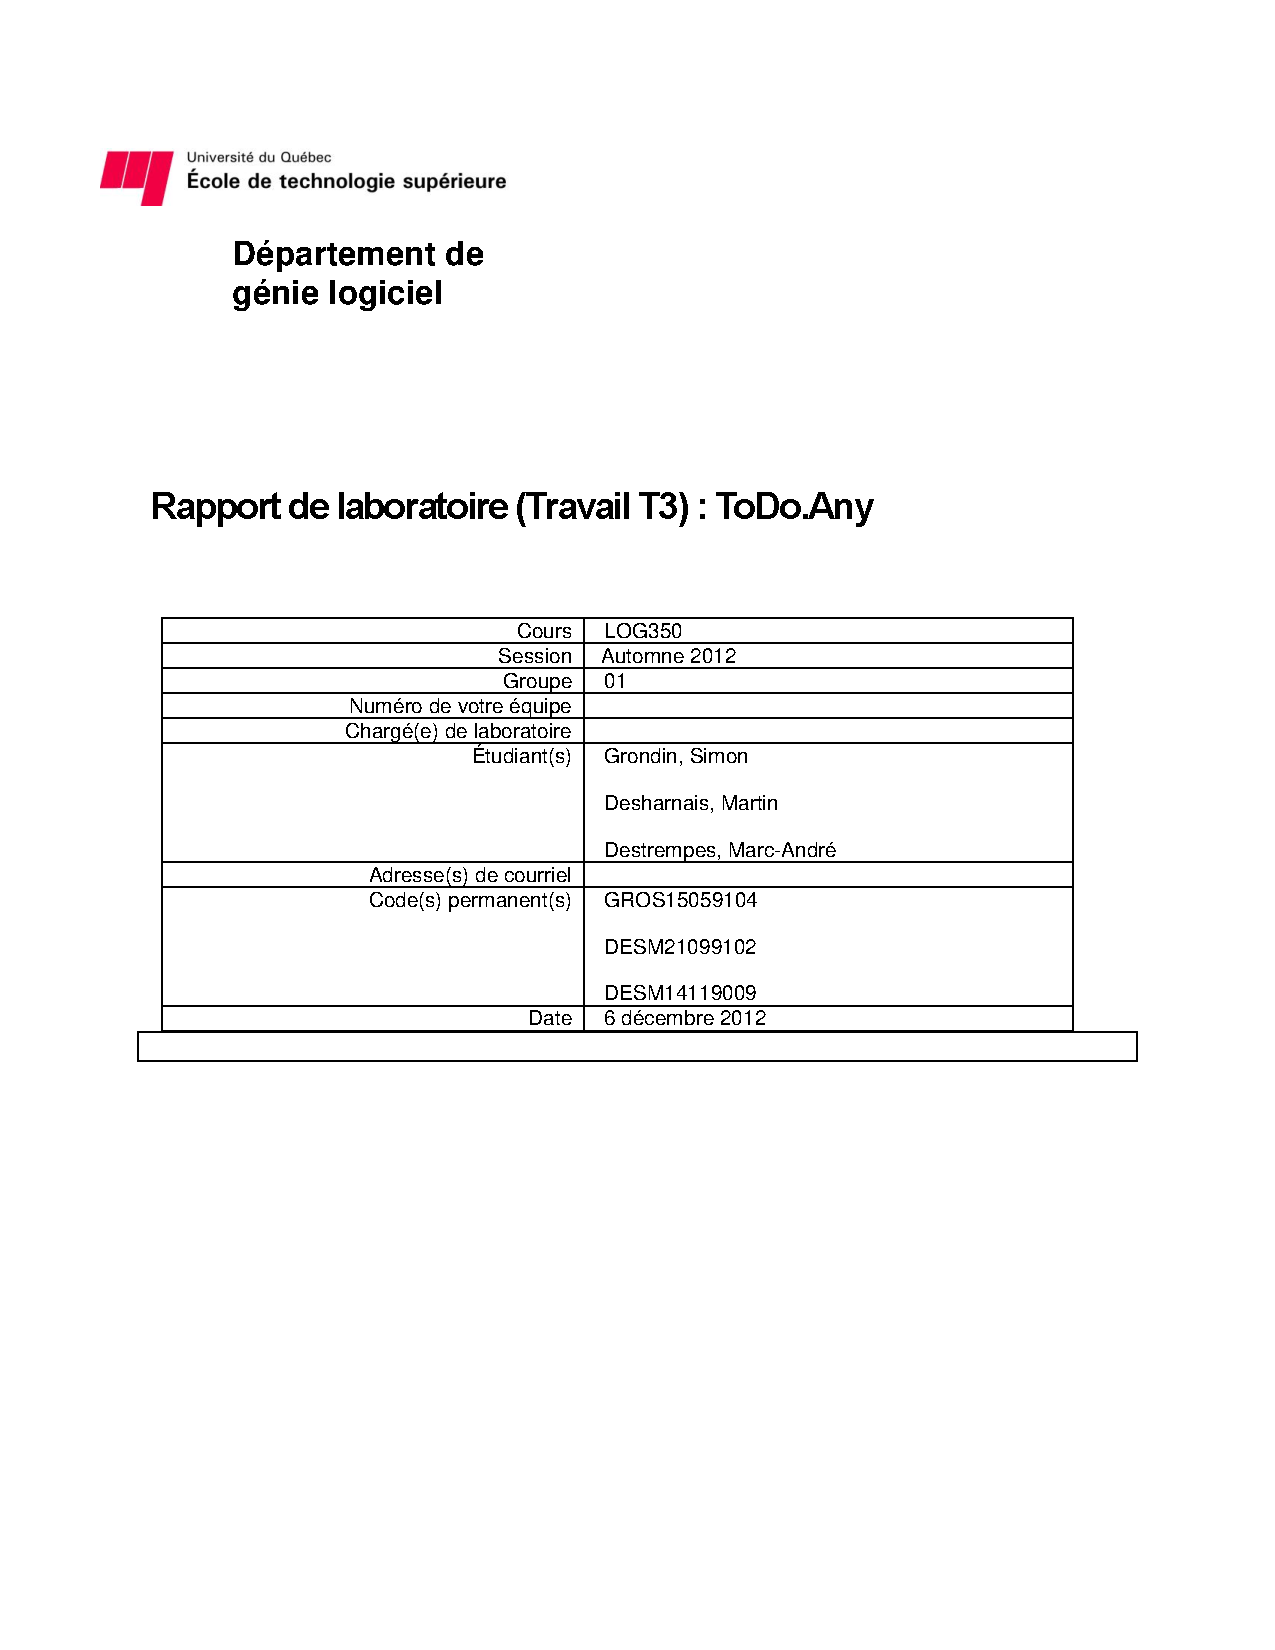
\includepdf[pages=-]{pageTitre.pdf}

\tableofcontents
\listoftables
\listoffigures

\chapter{Glossaire}

\begin{description}
\item[C\#] est un langage de programmation orienté objet à typage fort, créé par la société Microsoft. \footnote{\url{https://fr.wikipedia.org/wiki/C_sharp}}
\item[Windows Presentation Foundation (WPF)] est la spécification graphique de Microsoft .NET 3.0. Il intègre le langage descriptif XAML qui permet de l'utiliser d'une manière proche d'une page HTML pour les développeurs. \footnote{\url{https://fr.wikipedia.org/wiki/Windows_Presentation_Foundation}}
\item[WinForms] est le nom de l'interface graphique qui est incluse dans .NET Framework, fournissant l'accès via du Managed code à l'API Windows. \footnote{\url{https://fr.wikipedia.org/wiki/Windows_Forms}}
\item[framework] est un kit de composants logiciels structurels, qui sert à créer les fondations ainsi que les grandes lignes de tout ou d’une partie d'un logiciel (architecture). \footnote{\url{https://fr.wikipedia.org/wiki/Framework}}
\item[.NET 4.5] est un framework pouvant être utilisé par un système d'exploitation Microsoft Windows et Microsoft Windows Mobile depuis la version 5 (.NET Compact Framework). \footnote{\url{https://fr.wikipedia.org/wiki/Framework_.NET}}
\item[SQLite] est une bibliothèque écrite en C qui propose un moteur de base de données relationnelle accessible par le langage SQL.\footnote{\url{https://fr.wikipedia.org/wiki/SQLite}}
\item[Git] est un logiciel de gestion de versions décentralisé. C'est un logiciel libre créé par Linus Torvalds, le créateur du noyau Linux, et distribué selon les termes de la licence publique générale GNU version 2.\footnote{\url{https://fr.wikipedia.org/wiki/Git}}
\item[\LaTeX] est un langage et un système de composition de documents créé par Leslie Lamport en 1983. Plus exactement, il s'agit d'une collection de macro-commandes destinées à faciliter l'utilisation du « processeur de texte » TeX de Donald Knuth.\footnote{\url{https://fr.wikipedia.org/wiki/LaTeX}}
\end{description}

\chapter{Introduction et sommaire du travail effectué en TP2}

L'application permet la gestion simple de tâches et d'événements tout en offrant des fonctionnalités de gestion et de classification avancées. Parmi celles-ci, notons la possibilite de définir des rappels, de catégoriser les éléments, de définir un événement comme échéance d'une tâche ou encore de définir des sous-tâches à une tâche imposante.

Durant notre analyse de tâche, nous avons déterminer que le publique cible est des personnes de 15 ans et plus désirant organiser son temps et sa vie professionnelle. De plus, nous avons conclu que notre interface devrais ressembler à des interfaces connu pour la garder familière et garder une courbe d'apprentissage faible. Pour ce faire, nous avons dressé une liste des cas d'utilisation que l'application doit traiter pour se donner un point de départ. Par la suite, nous avons construit nos prototypes statiques.

Pour construire notre prototype statique, nous avons utilisé des fenêtres virtuelles où chaque point de chaque fenêtre à été détaillé pour s'assurer que le travail devant être effectué par chaque interface a bel et bien été compris. De plus, chaque fonctionnalité a aussi été détaillé dans le but qu'elles soient bien comprise.

Jusqu'à présent, presqu'aucune modification n'a été apporté entre les prototypes statiques et dynamiques sauf à quelques endroits pour des raisons de manque de temps et de personnel. Par exemple, dans la fenêtre Tâche, la section échéance a été changé. Pour le reste, tout va rester comme indiqué dans le document se trouvant à l'annexe III.

Dans le présent document, les tests qui seront effectués avec des utilisateurs seront listés et détaillés. Par la suite, un concensus sera fais pour chaque tâche et une amélioration qui pourrait être faite sera proposé pour améliorer le comportement du logiciel.

\chapter{Planification du travail}

\begin{table}
	\centering
	\begin{tabular}{|l|l|}
		\hline
		Semaine	& Travail accomplis 								\\ \hline
		4 novembre	& Choix de la technologie et apprentissage de celle-ci.		\\ \hline
		11 novembre	& Marc-André : Conception des interfaces. 				\\
				& Martin : Conception de la base de données.				\\
				& Simon : Conception de la base de données.				\\ \hline
		18 novembre	& Marc-André : Début de la rédaction du rapport. 			\\ 
				& Martin : Programmation du prototype dynamique. 			\\
				& Simon : Programmation du prototype dynamique. 			\\ \hline
		25 novembre	& Marc-André : Rédaction du rapport.		 			\\
				& Martin : Programmation du prototype dynamique. 			\\ 
				& Simon : Programmation du prototype dynamique.		 	\\ \hline
		2 décembre	& Marc-André : Rencontre avec les utilisateurs. 			\\
				& Martin : Préparation de la présentation.				\\
				& Simon : Préparation de la présentation.				\\ \hline
		9 décembre	& Marc-André : Rédaction du rapport.	 				\\ 
				& Martin : Rédaction du rapport.	 					\\ 
				& Simon : Rédaction du rapport.			 			\\ \hline
	\end{tabular}
	\caption{Échéancier}
\end{table}

\chapter{Réalisation du prototype dynamique}

Dans la section suivante, nous vous présenterons notre prototype dynamique et donc, avant d'entreprendre la lecture de cette section, nous vous conseillons de lire le document se trouvant à l'annexe III. Ce document contient les informations concernant le prototype statique et toute la logique derrière le prototype dynamique.

\section{Choix des outils}

Pour réaliser le prototype dynamique, nous avons décidé d'utiliser le C\# et le Windows Presentation Foundation (WPF) comme langages de programmation. Nous avons choisi ces langages tout simplement parce que ceci nous permet de séparer le code des interfaces et que le WPF va nous permettre de créer des composantes et de les implémenter dans notre interface personnalisé plus facilement. 

Comme environnement de développement, nous utilisons Visual Studio 2012 avec le framework .NET 4.5 pour faciliter et accélérer notre développement. Ce framework nous donne des composantes graphiques de base qui nous simplifie la vie en nous permettant d'économiser du temps pour ne pas à avoir à developper des composants de base comme un TextBox ou un Label, par exemple.

De plus, comme base de données, nous utilisons SQLite parce que cela nous permet d'avoir un endroit pour stocker nos données de façon structuré et le tout dans un seul et unique fichier. Ce qui nous permet d'avoir une base de données portable.

Pour assurer la gestion des versions, nous utilisons un logiciel connu sous le nom de Git.

Pour la production de la documentation, nous utilisons le processeur de texte \LaTeX.

\newpage

\section{Captures d'écran}

Dans la section suivante, nous ferons une brève description de chaque fenêtre de notre application. Cette description impliquera la description de chaques actions qui peuvent être effectuées ainsi qu'une capture d'écran pour permettre de visualiser les interactions.

\subsection{Fenêtre principale}

Cette fenêtre permet à l'utilisateur d'avoir la possibilité d'avoir plusieurs onglets pour organiser ces listes de tâches et d'événements et, dans de futures versions, effectuer des recherces pour afficher de l'information personnalisé dans ces onglets. Ensuite, pour faciliter l'ajout, un champ texte ainsi qu'un bouton Ajouter est mis à disposition pour effectuer un ajout rapide. Lorsque l'utilisateur à terminé d'ajouter, il peut faire la gestion de sa liste en modifiant les entrées en double cliquant ou bien en faisant apparaitre le menu contextuel pour supprimer. De plus, il faut spécifier que la gestion des priorités se fait via le bouton Configuration. À la page 16 et 18 du document, dans l'annexe III, il y a de plus ample informations concernant cette fenêtre.

\begin{figure}[H!]
	\centering
	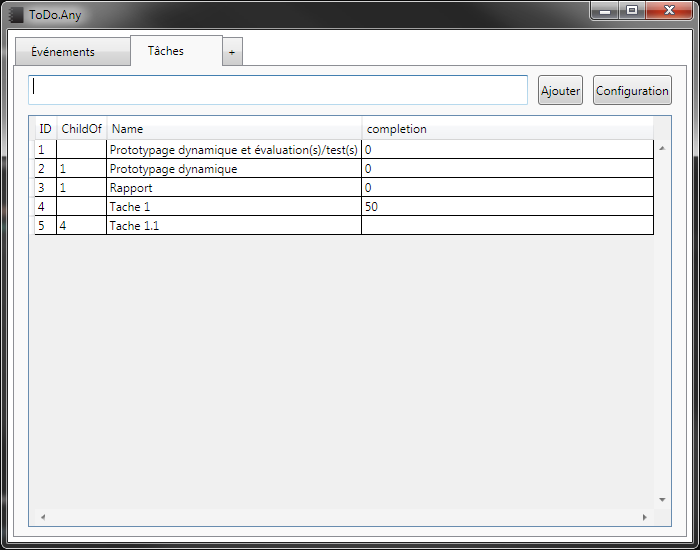
\includegraphics[width=1\textwidth]{fenetre_main.png}
	\caption{Fenêtre concernant la page principale}
\end{figure}

\newpage

\subsection{Événement}

Cette fenêtre permet à l'utilisateur d'entrer les diverses informations concernant un événement. Lorsque l'utilisateur modifie des informations le programme détecte automatiquement que quelque chose a changé et propose à l'utilisateur de sauvegarder les informations lorsque celui ferme la fenêtre. Si l'utilisateur décide d'ajouter une alerte, il n'a qu'à double cliquer dans la ligne vide pour effectuer un ajout. De plus, il peut modifier directement les alertes présentes et pour supprimer il n'a qu'a faire apparaitre le menu contextuel de chaque datagridview. À la page 21 du document, dans l'annexe III, il y a de plus ample informations concernant cette fenêtre.

\begin{figure}[H!]
	\centering
	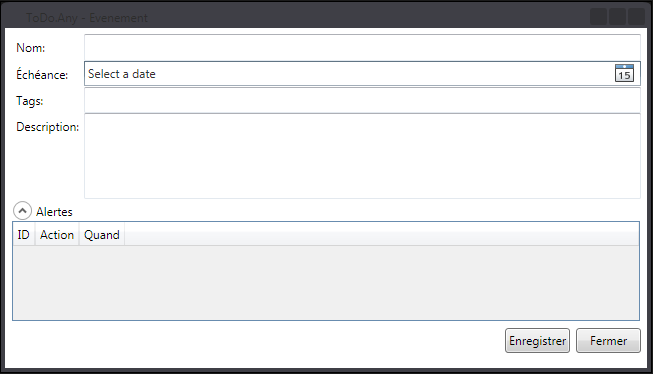
\includegraphics[width=1\textwidth]{fenetre_evenement.png}
	\caption{Fenêtre concernant un événement}
\end{figure}

\newpage

\subsection{Tâche}

Cette fenêtre permet à l'utilisateur d'entrer les diverses informations concernant une tâche. Lorsque l'utilisateur modifie des informations le programme détecte automatiquement que quelque chose a changé et propose à l'utilisateur de sauvegarder les informations lorsque celui ferme la fenêtre. Si l'utilisateur décide d'ajouter une alerte ou une sous-tâche, il n'a qu'à double cliquer dans la ligne vide pour effectuer un ajout. De plus, il peut modifier directement les alertes et sous-tâches présentes et pour supprimer il n'a qu'a faire apparaitre le menu contextuel de chaque datagridview. À la page 19 du document, dans l'annexe III, il y a de plus ample informations concernant cette fenêtre.

\begin{figure}[H!]
	\centering
	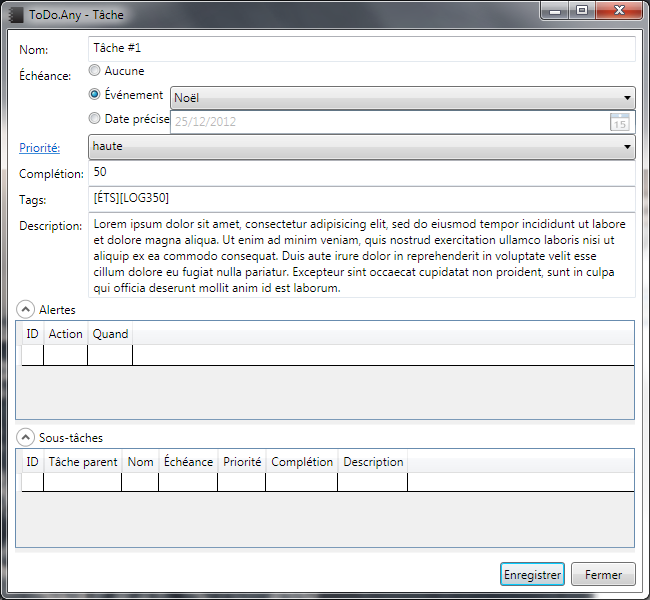
\includegraphics[width=1\textwidth]{fenetre_tache.png}
	\caption{Fenêtre concernant une tâche}
\end{figure}

\newpage

\subsection{Priorités}

Cette fenêtre permet à l'utilisateur de faire la gestion des diverses priorités.  Si l'utilisateur décide d'ajouter une priorité, il n'a qu'à double cliquer dans la ligne vide pour effectuer un ajout. De plus, il peut modifier directement les alertes présentes et pour supprimer il n'a qu'a faire apparaitre le menu contextuel de chaque datagridview. Pour ajouter À la page 22 du document, dans l'annexe III, il y a de plus ample informations concernant cette fenêtre.

\begin{figure}[H!]
	\centering
	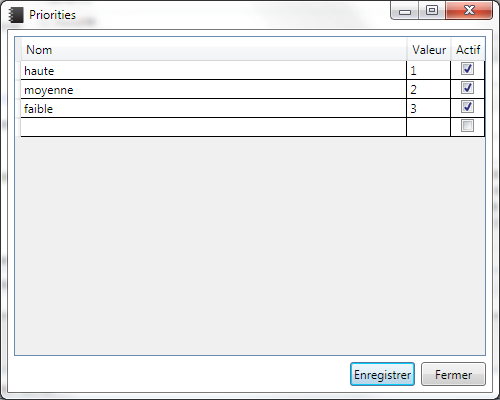
\includegraphics[width=1\textwidth]{fenetre_priorite.png}
	\caption{Fenêtre concernant les priorités}
\end{figure}

\newpage

\section{Justification des choix de conception}

Divers patrons de conception ont été utilisé pour parvenir à la conception de l'application que nous avons présentement. 

Parmi les divers patrons disponibles, on compte le patron \emph{Many Workspaces} qui se retrouve à la fenêtre principale de l'application ou l'utilisateur à la possibilite d'avoir plusieurs listes d'ouvertes et de les organiser comme il veut via des onglets. L'utilisateur peut donc gérer plusieurs listes à la fois. 

\begin{figure}[H!]
	\centering
	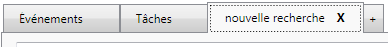
\includegraphics[width=1\textwidth]{many_workspaces.png}
	\caption{Onglets représentant différent espace de travail}
\end{figure}

Pour la navigation entre les fenêtres de l'application nous utilisons le patron \emph{Escape Hatch}. Ainsi, la navigation entre les fenêtres est limité et l'utilisateur peut toujours revenir a la fenêtre principale sans chercher pendant de longues minutes comment y revenir. Cela simplifie grandement l'interaction entre l'application et l'utilisateur en simplifiant le processus de navigation au maximum.

\begin{figure}[H!]
	\centering
	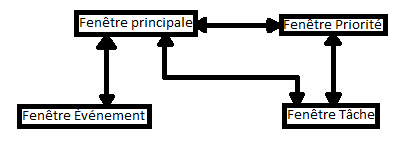
\includegraphics[width=1\textwidth]{navigation.png}
	\caption{Navigation entre les fenêtres}
\end{figure}

\newpage

Ensuite, pour ce qui est des listes, nous utilisons le patron \emph{Tree Table} sur, par exemple, la fenêtre principale. Avec ce patron, nous listons donc les tâches et chaque sous-tâche sous la tâche correspondante sous forme d'arborescence. Nous pouvons donc afficher un maximum d'information utile à l'utilisateur lorsque celui-ci le demande. Par manque de temps et de ressources humaines, ce patron a été implanté partiellement.

\begin{figure}[H!]
	\centering
	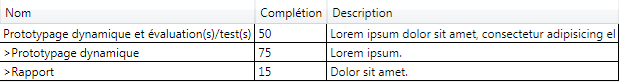
\includegraphics[width=1\textwidth]{tree_table.png}
	\caption{Datagridview avec le patron \emph{Tree Table}}
\end{figure}

Nous utilisons aussi le patron \emph{New-Item Row} dans la fenêtre Priorités, par exemple, pour permettre l'ajout rapide et infini de lignes dans le tableau sans que l'utilisateur n'ait besoin d'appuyer sur quoi que se soit. 

\begin{figure}[H!]
	\centering
	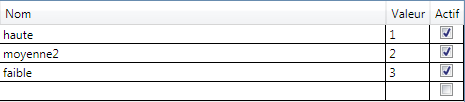
\includegraphics[width=1\textwidth]{new_item_row.png}
	\caption{Datagridview avec le patron \emph{New-Item Row}}
\end{figure}

Pour ce qui est de toutes les grilles, le patron \emph{Sortable Table} s'applique et permet de trier l'information affiché en tout temps pour permettre à l'utilisateur de trouver ce qu'il veut plus rapidement.

\begin{figure}[H!]
	\centering
	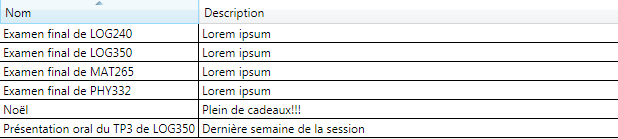
\includegraphics[width=1\textwidth]{sortable_table.png}
	\caption{Exemple d'une colonne trié}
\end{figure}

De plus, nous avons respecté le plus possible le contenu de la norme \emph{ISO 9241-120} à \emph{ISO 9241-129} qui traite sur les interactions sur les entrées, les sorties et les interactions.

Quelques changements on été effectué entre le prototype statique et dynamique. Parmi ces changements, on compte les options possibles pour une échéance dans la fenêtre sur les tâches. Ce changement a été fait à cause de limitations logiciels et par faute de temps. Il est à noter que ces changements n'influence en aucun cas l'efficacité de l'application.

\section{Améliorations possibles}

Quelques améliorations possibles seraient d'utiliser les lois psychomotrices de Fitts et Miller pour optimiser l'interface. Nous pourrions ainsi optimiser les déplacements que l'utilisateur doit faire avec sa souris pour cliquer sur les boutons et les champs de saisies dans les fenêtres. Mais, par faute de temps et de ressources humaines, il nous est donc impossible d'effectuer ces tests.

\chapter{Démonstration du prototype dynamique en laboratoire}

Un prototype dynamique de l'application est disponible à l'adresse suivante : \\
\url{https://github.com/xeph/LOG350.TP3}.

Évaluation du prototype en laboratoire  : le 4 décembre 2012 au laboratoire (pour les 2 groupes).

Exposé oral  : le 6 décembre 2012 dans un local à définir (pour les 2 groupes).

Remise du code final : le 11 décembre 2012 à 23h59 maximum par courriel à log350a2012@gmail.com.

Remise du rapport :  le 11 décembre 2012 à 23h59 maximum en version papier dans la chute du département.

Remise de la présentation de l’exposé oral : le 6 décembre 2012 à 23h59 maximum par courriel à log350a2012@gmail.com.

\chapter{Tests avec utilisateurs}

\section{Méthodologie}

Avant d'effectuer les tests, un document expliquant la nature du projet et le déroulement des tests a été fourni aux utilisateurs. Les membres de l'équipe assument que le document a été lu lors de la rencontre. De plus, un formulaire de consentement sera obligatoirement signé par l'utilisateur et un membre de l'équipe pour que les deux parties s'entendent sur ce qui sera fait lors de la rencontre.

Pour faire les tests avec les utilisateurs, le ou les membres de l'équipe s'asseoiront avec l'utilisateur qui testera l'application. Par la suite, un membre de l'équipe se chargera de dire chaque tâche que l'utilisateur devra effectuer, et si l'utilisateur à des questions, il sera chargé de lui fournir les informations. Lorsque l'utilisateur aura terminé de faire une tâche, il y aura une brève pause pour que tout le monde ait le temps de prendre des notes. L'exécution de la tâche suivante se fera lorsque tout le monde aura terminer de prendre les notes pour la tâche courante. Quand toutes les tâches auront été exécuté, l'utilisateur pourra donner son opinion et ses impressions sur l'application sur des choses à améliorer, les points positifs et des fonctionnalitées qui pourraient être intéressante à ajouter ou bien améliorer.

Ce seront principalement des notes concernant la performance et l'usabilité de l'application qui seront prise parce que les principaux objectifs que nous voulons atteindre avec notre application sont une facilité d'utilisation et que celle-ci soit performante. Les notes seront tirées de l'interaction de l'utilisateur avec l'application et de la rapidité avec laquelle l'utilisateur effectue les tâches.

Les tests se feront dans le calme et le respect. De plus, l'utilisateur peut, en tout temps, décider d'arrêter les tests sans devoir fournir une raison. Les données recueillis seront cependant conservé à moins que l'utilisateur ne demande à ce qu'elles soient détruites.

\newpage

\section{Liste des tâches}

\begin{table}
	\centering
	\begin{tabular}{|l|l|l|}
		\hline
		no Tâche	& Titre et description		& Éléments que vous voulez vérifier et hypothèses 	\\ \hline 
		1		& Ajouter l'événement 		&  Détection de raccourcis.				\\ 
				& « événement 1 ».			&								\\ \hline
		2		& Définir l’échéance de 		&								\\
				& « événement 1 » à 1 		&								\\
				& janvier 2013.			&								\\ \hline
		3		& Ajouter le tag « [TAG1] » 	&								\\
				& à « événement 1 ».		&								\\ \hline
		4		& Ajouter une alerte « Envoyer 	&								\\
				& un courriel », « 2 », « jours ».	&								\\ \hline
		5		& Enregistrer l’événement.	& 								\\ \hline
		6		& Fermer la fenêtre.		&								\\ \hline
		7		& Supprimer l’événement		& Détection de menu contextuel.				\\
				&  « Examen final de PHY332 ».	& 								\\ \hline
		8		& Ajouter la tâche « tâche 1 ». 	& Détection de raccourcis.					\\ \hline
		9		& Définir l’échéance de  		&								\\
				& « tâche 1 » comme étant	&								\\
				&  l’événement « événement 1 ».	&								\\ \hline
		10		& Définir la priorité de  « tâche 1 »& Détection de raccourcis.				\\
				&  à « Très faible ». 		&								\\
				& <NE PEUT PAS ÊTRE FAIT>	&								\\ \hline
		11		& Ajouter la priorité « très faible »&								\\
				& avec une valeur de « 4 » et 	&								\\
				& Actif à « Vrai » et enregistrer.	&								\\ \hline
		12		& Définir la priorité de  « tâche 1 »&								\\
				&  à « Très faible »..		&								\\ \hline
		13		& Définir la complétion de 		&								\\
				& « tâche 1 » à « 42 ».		&								\\ \hline
		14		& Ajouter les tags « [TAG1] » et 	&								\\
				& « [TAG2] » à « tâche 1 ».	&								\\ \hline
		15		& Ajouter la description 		&								\\
				& « lorem ipsum » à « tâche 1 ».	&								\\ \hline
		16		& Ajouter une alerte 	 	&								\\
				& « afficher un rappel », « 5 »,	& 								\\
				&  « minutes » à « tâche 1 ».	&								\\ \hline
		17		& Créer une sous-tâche		&								\\
				&  « tâche 1.1 » à « tâche 1 »	&								\\ \hline
		18		& Créer une sous-tâche		&								\\
				&  « tâche 1.2 » à « tâche 1 »	&								\\ \hline
		19		& Enregistrer la tâche.		& 								\\ \hline
	\end{tabular}
\end{table}

\newpage

\begin{table}
	\centering
	\begin{tabular}{|l|l|l|}
		\hline
		no Tâche	& Titre et description		& Éléments que vous voulez vérifier et hypothèses 	\\ \hline 
		20		& Fermer la fenêtre.		&								\\ \hline
		21		& Supprimer la « tâche 1.2 »	&								\\ \hline
		22		& Modifier l’échéance de « tâche 1 »&								\\
				&  pour le « 3 février 2013 ».	&								\\ \hline
		23		& Fermer la fenêtre.		&								\\ \hline
		24		& Appuyer sur « Cancel ».		&								\\ \hline
		25		& Définir la complétion de la 	&								\\
				& « tâche 1 » à « 50 ».		&								\\ \hline
		26		& Fermer la fenêtre.		&								\\ \hline
		27		& Appuyer sur « Oui ».		&								\\ \hline
		28		& Appuyer sur le bouton 		&								\\
				& « Configuration ».		&								\\ \hline
		29		& Définir la priorité « très faible » &								\\
				& à « non-actif »			&								\\ \hline
		30		& Fermer la fenêtre.		&								\\ \hline
		31		& Appuyer sur « Oui ».		&								\\ \hline
		32		& Modifier la priorité de la 		&								\\
				& « tâche 1 » à « faible ».		&								\\ \hline
		33		& Enregistrer la tâche.		&								\\ \hline
		34		& Fermer la fenêtre.		&								\\ \hline
	\end{tabular}
	\caption{Liste des tâches}
\end{table}

\section{Liste des utilisateurs}

Les caractéristiques principales des utilisateurs choisis sont la gestion de leurs tâches pour les travaux et devoirs au CEGEP ou bien à l'université et la gestion des rendez-vous pour les professionnels. Nous avons choisis ce nombre d'utilisateur, car il nous fallait un petit échantillon oeuvrant dans le même type de vie que le publique visée mais dans des sphères professionnelles différentes. Il est pertinant d'avoir testé avec ces utilisateurs parce que se sera principalement ce type d'utilisateur qui se servira d'une application comme celle-ci.

\newpage

\section{Résultats}

\begin{table}
	\centering
	\begin{tabular}{|l|l|l|}
	\hline
	no Tâche	& Points importants de l'observation	\\ \hline
	1		& a ajouté une ligne vide et double	\\ 
			& cliquer sur l'entrée ensuite		\\ \hline
	2		& 						\\ \hline
	3		& 						\\ \hline
	4		& a pesé sur	$\bigtriangleup$ en $1^{er}$ \\
			& n'entre pas le 2 (date à la place)	\\ \hline
	5		& 						\\ \hline
	6		& 						\\ \hline
	7		& ne trouve pas coment supprimer	\\ \hline
	8		& n'utilise pas la barre d'ajout rapide	\\ \hline
	9		& 						\\ \hline
	10		& 						\\ \hline
	11		& 						\\ \hline
	12		& 						\\ \hline
	13		& 						\\ \hline
	14		& ; au lieu de les coller			\\ \hline
	15		& 						\\ \hline
	16		& 						\\ \hline
	17		& 						\\ \hline
	18		& 						\\ \hline
	19		& 						\\ \hline
	20		& 						\\ \hline
	21		& 						\\ \hline
	22		& 						\\ \hline
	23		& 						\\ \hline
	24		& 						\\ \hline
	25		& 						\\ \hline
	26		& 						\\ \hline
	27		& 						\\ \hline
	28		& 						\\ \hline
	29		& 						\\ \hline
	30		& 						\\ \hline
	31		& 						\\ \hline
	32		& 						\\ \hline
	33		& 						\\ \hline
	34		& 						\\ \hline
	\end{tabular}
	\caption{Résultats de l'utilisateur 1}
\end{table}

\newpage

\begin{table}
	\centering
	\begin{tabular}{|l|l|l|}
	\hline
	no Tâche	& Points importants de l'observation	\\ \hline
	1		& n'utilise pas la barre d'ajout rapide	\\ \hline
	2		& 						\\ \hline
	3		& 						\\ \hline
	4		& a pesé sur	$\bigtriangleup$ en $1^{er}$ \\ \hline
	5		& 						\\ \hline
	6		& 						\\ \hline
	7		& ne trouve pas coment supprimer	\\ \hline
	8		& ne trouve pas tâche			\\ \hline
	9		& 						\\ \hline
	10		& 						\\ \hline
	11		& 						\\ \hline
	12		& 						\\ \hline
	13		& 						\\ \hline
	14		& 						\\ \hline
	15		& 						\\ \hline
	16		& 						\\ \hline
	17		& 						\\ \hline
	18		& 						\\ \hline
	19		& 						\\ \hline
	20		& 						\\ \hline
	21		& 						\\ \hline
	22		& 						\\ \hline
	23		& 						\\ \hline
	24		& 						\\ \hline
	25		& 						\\ \hline
	26		& 						\\ \hline
	27		& 						\\ \hline
	28		& 						\\ \hline
	29		& changer le nom au lieu du check box	\\ \hline
	30		& 						\\ \hline
	31		& 						\\ \hline
	32		& 						\\ \hline
	33		& 						\\ \hline
	34		& 						\\ \hline
	\end{tabular}
	\caption{Résultats de l'utilisateur 2}
\end{table}

\newpage

\section{Discussion et recommandations}

\begin{table}
	\centering
	\begin{tabular}{|l|l|l|}
	\hline
	no Tâche	& Résumé	& Recommandation 	\\ \hline
	1		&  n'utilise pas la barre d'ajout rapide		&  mettre la barre plus visible			\\ \hline
	2		& 							&  							\\ \hline
	3		& 							&  							\\ \hline
	4		&  a pesé sur	$\bigtriangleup$ en $1^{er}$	&  remplacer les expander par des groupbox	\\ \hline
	5		& 							&  							\\ \hline
	6		& 							&				  			\\ \hline
	7		& ne trouve pas coment supprimer		&  fournir un bouton supprimer			\\ \hline
	8		& 							&  							\\ \hline
	9		& 							&  							\\ \hline
	10		& 							&  							\\ \hline
	11		& 							&  							\\ \hline
	12		& 							&  							\\ \hline
	13		& 							&  							\\ \hline
	14		& 							&  							\\ \hline
	15		& 							&  							\\ \hline
	16		&							&  							\\ \hline
	17		& 							&  							\\ \hline
	18		& 							&  							\\ \hline
	19		& 							&  							\\ \hline
	20		& 							&  							\\ \hline
	21		& 							&  							\\ \hline
	22		& 							&  							\\ \hline
	23		& 							&  							\\ \hline
	24		& 							&  							\\ \hline
	25		& 							&  							\\ \hline
	26		& 							&  							\\ \hline
	27		& 							&  							\\ \hline
	28		& 							&  							\\ \hline
	29		& 							&  							\\ \hline
	30		& 							&  							\\ \hline
	31		& 							&  							\\ \hline
	32		& 							&  							\\ \hline
	33		& 							&  							\\ \hline
	34		& 							&  							\\ \hline
	\end{tabular}
	\caption{Recommandations par les observateurs}
\end{table}

\newpage

\begin{table}
	\centering
	\begin{tabular}{|l|l|l|}
	\hline
	no Tâche	& Résumé	& Recommandation 	\\ \hline
	1		&  n'utilise pas la barre d'ajout rapide		&  modifier la barre d'ajout						\\ \hline
	2		& 							&  									\\ \hline
	3		& 							&  									\\ \hline
	4		&  a pesé sur	$\bigtriangleup$ en $1^{er}$	&  ne comprends pas le fonctionnement				\\ \hline
	5		& 							&  									\\ \hline
	6		& 							&  									\\ \hline
	7		& ne trouve pas coment supprimer		&  changer l'endroit ou se trouve supprimer			\\ \hline
	8		& 							&  									\\ \hline
	9		& 							&  									\\ \hline
	10		& 							&  									\\ \hline
	11		& 							&  									\\ \hline
	12		& 							&  									\\ \hline
	13		& 							&  									\\ \hline
	14		& 							&  									\\ \hline
	15		& 							&  									\\ \hline
	16		&							&  									\\ \hline
	17		& 							&  									\\ \hline
	18		& 							&  									\\ \hline
	19		& 							&  									\\ \hline
	20		& 							&  									\\ \hline
	21		& 							&  									\\ \hline
	22		& 							&  									\\ \hline
	23		& 							&  									\\ \hline
	24		& 							&  									\\ \hline
	25		& 							&  									\\ \hline
	26		& 							&  									\\ \hline
	27		& 							&  									\\ \hline
	28		& 							&  									\\ \hline
	29		& 							&  									\\ \hline
	30		& 							&  									\\ \hline
	31		& 							&  									\\ \hline
	32		& 							&  									\\ \hline
	33		& 							&  									\\ \hline
	34		& 							&  									\\ \hline
	\end{tabular}
	\caption{Recommandations par les utilisateurs}
\end{table}

La barre d'ajout rapide plante dans un nouvel onglet (SearchTasks.xaml.cs), les bugs n'ont pu être reproduit.

\chapter{Changements recommandés}

Fournir un menu d'aide (tooltip par exemple) explicant diverses fonctionnalités qui ne sont pas toujours évidente pour l'utilisateur, comme le système de tag ou bien les menus contextuel. Ainsi, l'utilisateur ne se sentira pas abandonné pour utiliser l'application et ceci facilitera aussi son apprentissage des diverses fonctionnalitées de l'application.

\begin{figure}[H!]
	\centering
	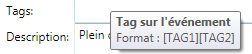
\includegraphics[width=1\textwidth]{tags.png}
	\caption{Exemple de tooltip sur le champ tag}
\end{figure}

Ajouter un bouton ajouter et supprimer en bas à gauche de chaque datagridview permettant l'ajout et la suppression des éléments dans celui-ci en plus du menu contextuel. En faisant cela, on offre la possibilité, tant aux utilisateurs débutants qu'aux utilisateurs avancés, d'ajouter et de supprimer un élément de diverses facon selon les préférences de chacun. Cela permet aussi à l'utilisateur de moins chercher comment effectuer cette opération.

\begin{figure}[H!]
	\centering
	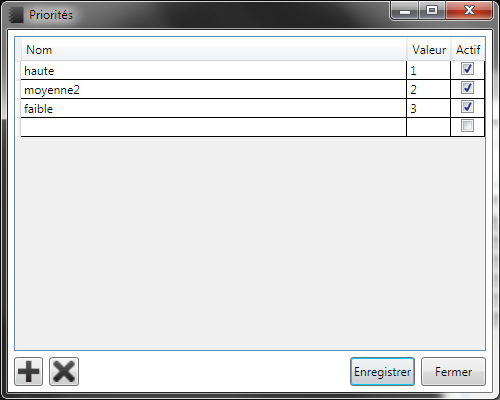
\includegraphics[width=0.6\textwidth]{add_delete_button.png}
	\caption{Boutons ajouter et supprimer sur un datagridview}
\end{figure}

\newpage

Changer le champ complétion dans la fenêtre tâche pour un slider, comme sa l'utilisateur ne pourra pas entrer ce qu'il veut. En faisant cela, on évite qu'une complétion ait au dessus de 100\% et au-dessous de 0\%, ce qui serais complètement illogique. L'utilisateur trouvera aussi plus intuitif d'utiliser ce composant, car il n'aura qu'a glisser jusqu'au niveau de complétion qu'il désire au lieu de l'écrire manuellement et de ce tromper.

\begin{figure}[H!]
	\centering
	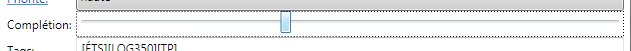
\includegraphics[width=1\textwidth]{completion.png}
	\caption{Slider de complétion}
\end{figure}

Changer les expander pour des groupbox, car avec les tests utilisateurs, nous nous sommes rendu compte que ceux-ci n'étaient pas familié avec ce type de composant et qu'aucun d'eux ne savait quoi faire avec ceci. Donc, pour simplifier le fonctionnement de la fenêtre et diminuer son temps d'apprentissage, il vaut mieux faire ce changement.

\begin{figure}[H!]
	\centering
	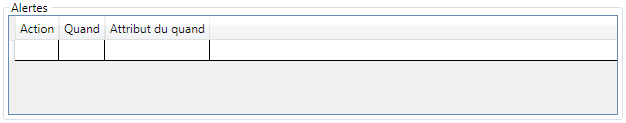
\includegraphics[width=1\textwidth]{groupbox.png}
	\caption{Groupbox au lieu d'expander}
\end{figure}

Selon les conclusions tirées des tests utilisateurs, la barre d'ajout rapide n'a pas été utilisé pour faire l'ajout rapide. Pour que les utilisateurs débutants puissent connaître cette fonctionnalité, il sera nécessaire d'inclure une fenêtre d'aide pour spécifier chaque action possible dans une fenêtre comme dans cet image.

\begin{figure}[H!]
	\centering
	
\includegraphics[width=0.48\textwidth]{help.png}
	\caption{Exemple de fenêtre d'aide}
\end{figure}

\chapter{Conclusion}

En conclusion, ce projet a été l'occasion de faire une incartade dans le monde du développement d'interfaces utilisateurs. Nous avons eu l'occasion de participer et d'en apprendre plus sur les différentes étapes de conception : analyse de tâches, prototype statique et prototype dynamique.

D'abord, l'analyse de tâches et le prototype statique nous ont amenés à comprendre l'importance de bien connaître son public afin de produire des interfaces utilisateurs qui correspondent réellement à ses besoins. Pour ce faire, nous avons utilisé le vieux principe d'être notre propre public cible. Nous nous sommes demandé quels sont les besoins que nous avions pour gérer notre emploi du temps efficacement et avons tenté de concevoir un système qui réponde à ces exigences. Nous sommes partis du principe que, si nous arrivions à produire un logiciel qui réponde à nos propres besoins, le projet pourrait être considéré comme une réussite.

Par la suite, nous nous sommes demandé si une telle application pouvait être utile à un auditoire plus élargi. Nous avons présenté notre concept et nos idées à des personnes tierces et avons recueilli leurs commentaires et réactions afin de peaufiner quelques détails. Cette expérience nous a confortés dans notre idée que, si des concepteurs connaissent bien leurs utilisateurs et arrivent à penser comme eux, le système produit est plus adapté et plus cohérent.

Ensuite, la réalisation du prototype dynamique nous a appris l'importance, pour un développeur, de bien connaître ses outils avant de s'engager dans la conception d'un système. Au début du projet, nous avons décidé d'utiliser la bibliothèque graphique WPF, une technologie nouvelle pour nous, et nous sommes dit que nous l'apprendrions au fils de l'avancement du projet. Ceci s'est avéré plus difficile que prévu.

Il s'est d'abord avéré assez rapide et facile de faire fonctionner une interface simple utilisant les composants fournis de base. Malheureusement, la situation s'est complexifiée lorsque nous avons voulu implémenter des interfaces nécessitant des composants qui n'existent pas dans la bibliothèque. Toutes les briques nécessaires pour construire de tels composants sont disponibles, mais acquérir les compétences pour développer de nouveaux contrôles WPF prend beaucoup plus de temps que ce que nous avions à notre disposition.

Le meilleur exemple de ces difficultés rencontrées est le système multionglets. Dans la phase d'analyse et de réalisation du prototype statique, nous avions l'intention d'offrir la possibilité de définir des vues plus spécialisées de la liste de tâches dans des onglets supplémentaires. Il aurait alors été possible de créer une vue qui n'affiche que les tâches concernant l'université ou bien uniquement les tâches qui doivent être complétées dans les 48 prochaines heures. Malheureusement, il a fallu tellement de temps pour réussir à implémenter un contrôle permettant à l'utilisateur de créer et supprimer des onglets que nous n'avons pas eu le temps et les ressources nécessaires pour implémenter la fonctionnalité de requête pour configurer une vue.

Enfin, il est ressorti de nos différentes conversations avec des utilisateurs que plusieurs trouvaient l'application visuellement « ordinaire », mais qu'aucun n'avait la même opinion de ce qui permettrait de la rendre plus « belle ». Parmi les membres de notre équipe, aucun ne se considère comme un artiste et ne sait comment créer un arrangement de formes et de couleurs qui plairait à une majorité. Cette constatation met de l'avant le fait qu'il y a une différence importante entre développer une interface efficace et une interface visuellement attirante. Le cours que nous avons suivi tente de nous apprendre à développer la première, mais ne prétend nullement nous apprendre à développer la seconde.

Concernant le cours, nous suggérons que celui-ci donne une plus grande place aux applications dites de bureau. Celles-ci étant encore très présentes comme applications « grand public » et largement dominantes dans le monde professionnel, il serait intéressant qu'elles occupent une plus grande place. Certaines sont très simples d'utilisation alors que d'autres sont incroyablement complexes. Qu'est-ce qui les distingue? Quelles sont les bonnes habitudes à imiter? Quelles sont les erreurs à ne pas commettre?

\appendix
\multiannexe

\chapter{Formulaire de consentement des utilisateurs}


\includepdf[pages=-]{form.pdf}

\chapter{Document de présentation du projet}

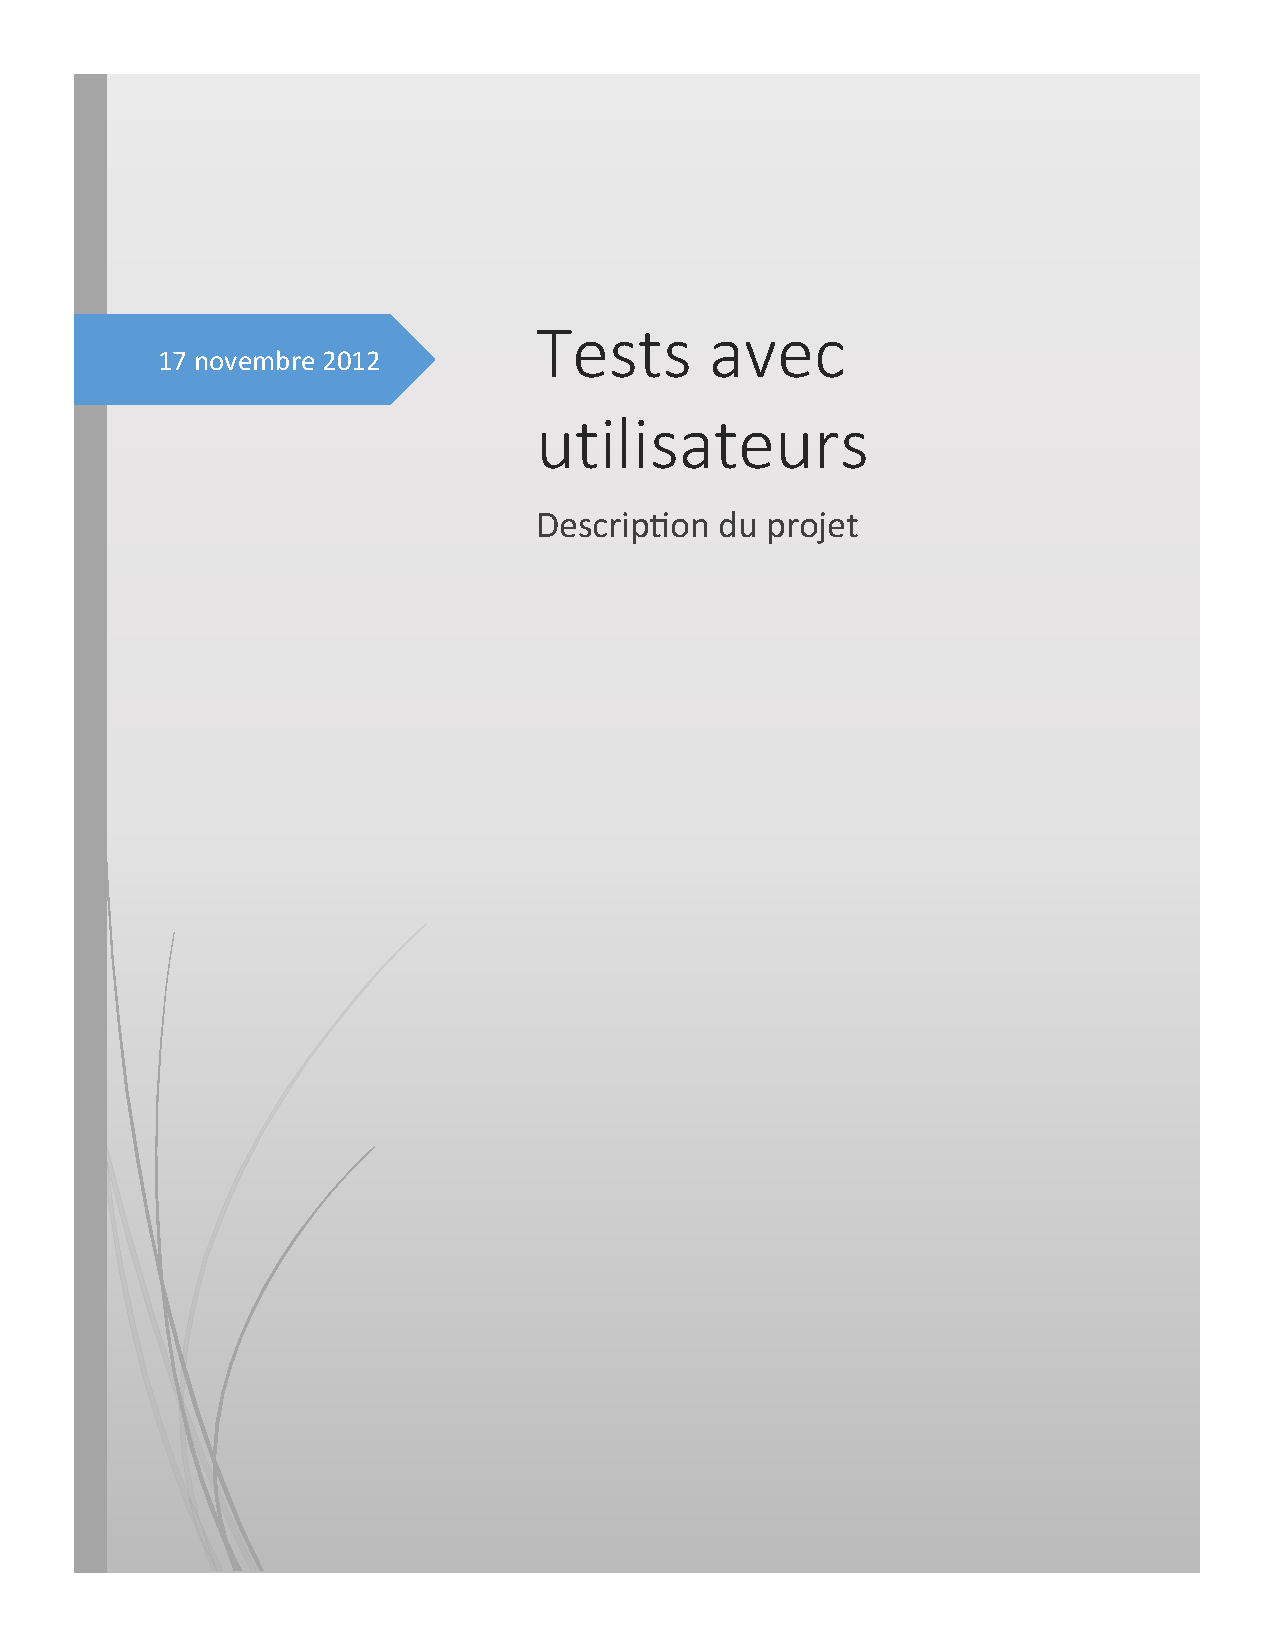
\includepdf[pages=-]{document.pdf}

\chapter{Travail Pratique 2}

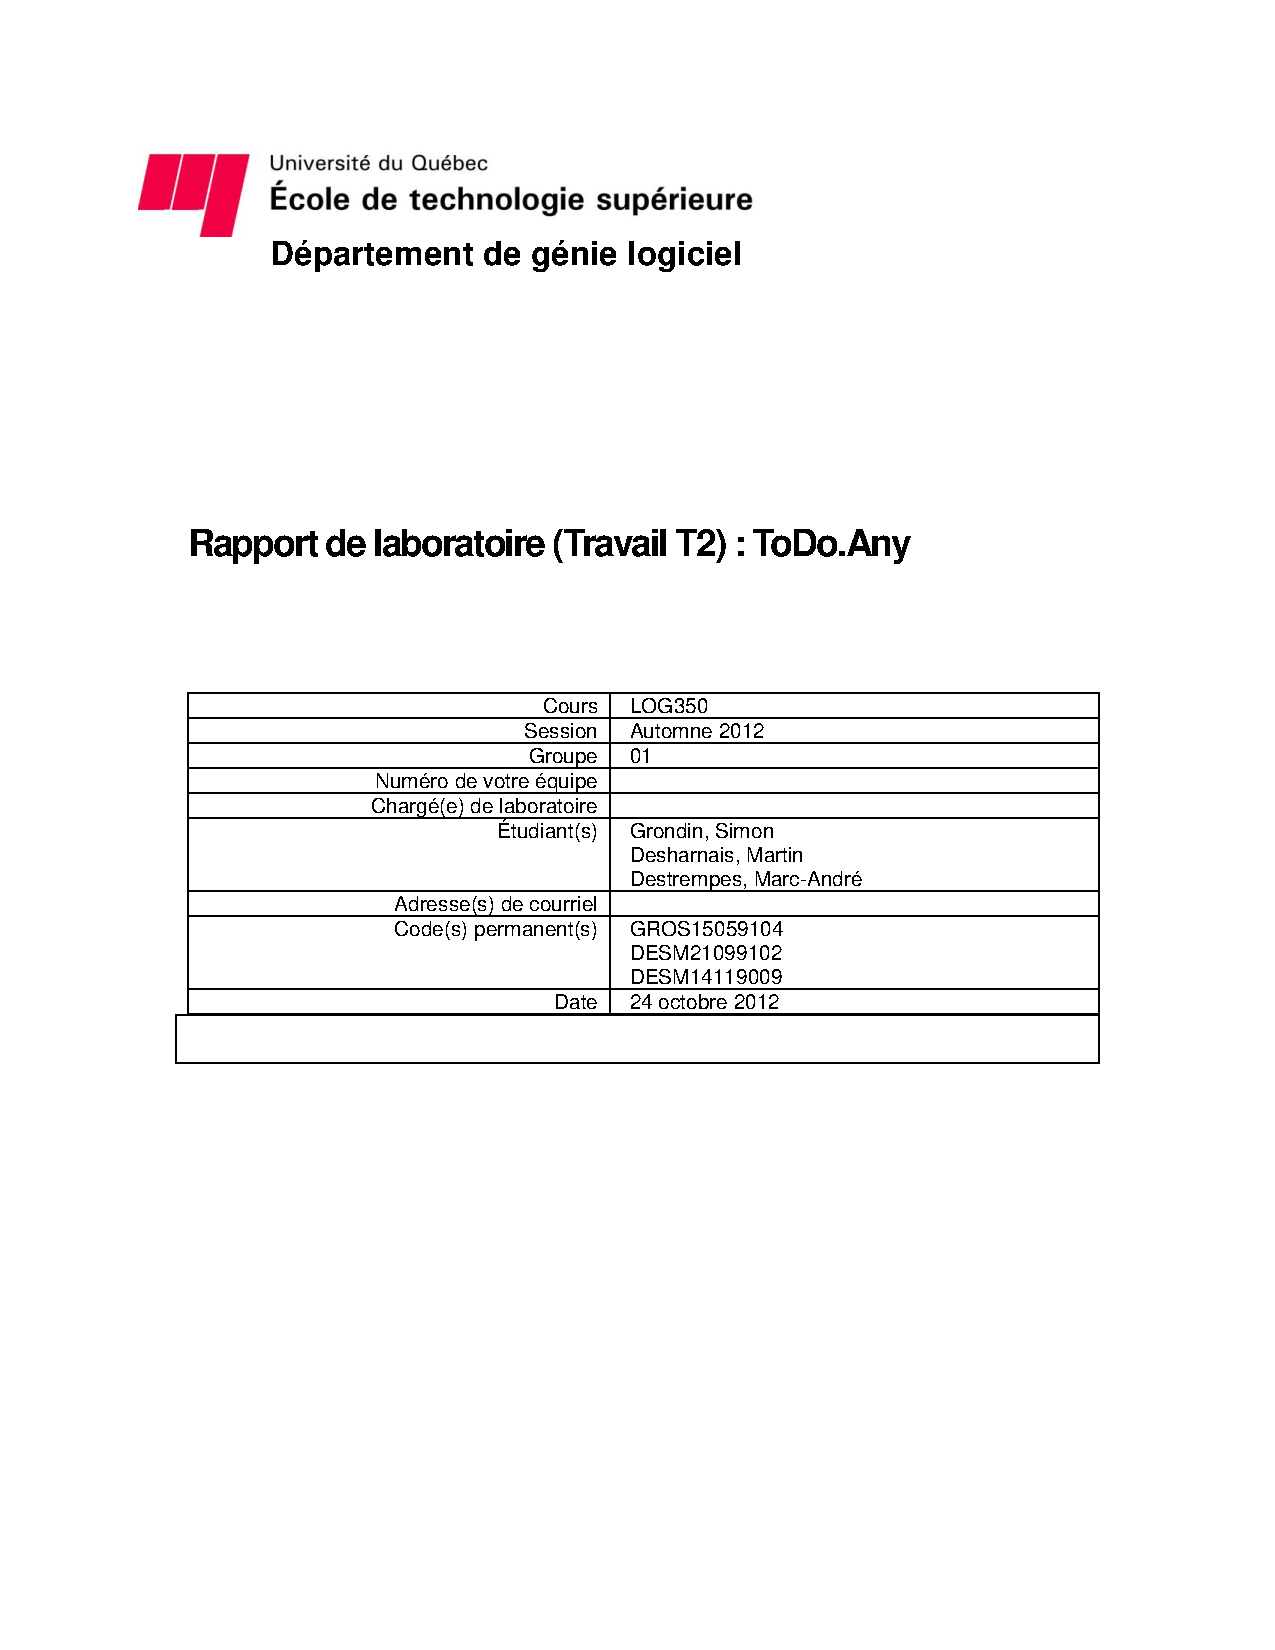
\includepdf[pages=-]{T2.pdf}

\chapter{Contrats signés}

%includedpdf[pages=-]{contrats_signes.pdf}

\chapter{Notes prises}

%includedpdf[pages=-]{notes_prises.pdf}

\end{document}
